% \documentclass[table]{beamer}
\documentclass[table,handout]{beamer}
\setbeameroption{show notes}
% \setbeameroption{hide notes}
% \setbeameroption{show only notes}
\usepackage{varwidth}

\newif\ifhide
\newif\ifpost
\newif\ifhideclicker

% \hidetrue
% \hideclickertrue
% \posttrue

\newcommand{\whiteout}[1]{\textcolor{white}{#1}}
% \newcommand{\whiteoutbox}[1]{\fcolorbox{white}{white}{\parbox{\dimexpr \linewidth-2\fboxsep-2\fboxrule}{\whiteout{#1}}}}
% \newcommand{\notebox}[1]{\fcolorbox{blue}{white}{\parbox{\dimexpr \linewidth-2\fboxsep-2\fboxrule}{#1}}}
\newcommand{\whiteoutbox}[1]{\fcolorbox{white}{white}{\parbox{\linewidth}{\whiteout{#1}}}}
\newcommand{\notebox}[1]{\fcolorbox{blue}{white}{\parbox{\linewidth}{#1}}}
\newcommand{\blankbox}[1]{\phantom{\varwidth{\linewidth}\whiteoutbox{#1}\endvarwidth}}
\newcommand{\blank}[1]{\phantom{\varwidth{\linewidth}#1\endvarwidth}}

\ifhide%
    \newcommand{\hmask}[1]{\blank{#1}}%
\else%
    \newcommand{\hmask}[1]{#1}%
\fi

\ifhide%
    \newcommand{\wout}[1]{\whiteout{#1}}%
\else%
    \newcommand{\wout}[1]{#1}%
\fi

\ifhide%
    \newcommand{\hignore}[1]{}%
\else%
    \newcommand{\hignore}[1]{#1}%
\fi

\ifpost%
    \newcommand{\nopost}[1]{}%
\else%
    \newcommand{\nopost}[1]{#1}%
\fi

\ifhideclicker%
    \newcommand{\clickerslide}[1]{\stepcounter{clickerQuestionCounter}%
        \begin{frame}[t]
            \textcolor{blue}{Q \arabic{clickerQuestionCounter}:}
        \end{frame}}
\else%
    \newcommand{\clickerslide}[1]{#1}%
\fi

\ifhide%
    \newcommand{\hidebox}[1]{\blank{#1}}%
\else%
    \newcommand{\hidebox}[1]{\notebox{#1}}%
\fi

\ifhide%
    \newcommand{\wbox}[1]{\whiteoutbox{#1}}%
\else%
    \newcommand{\wbox}[1]{\notebox{#1}}%
\fi

\ifhide%
    \newcommand{\nbox}[1]{\blankbox{#1}}%
\else%
    \newcommand{\nbox}[1]{\notebox{#1}}%
\fi

\ifhideclicker%
    \newcommand{\clickeranswer}[1]{#1}%
\else%
    \ifhide%
        \newcommand{\clickeranswer}[1]{#1}%
    \else%
        \newcommand{\clickeranswer}[1]{\textbf{\textcolor{blue}{#1}}}%
    \fi
\fi

\usepackage{beamerthemesplit}
% \usetheme{boxes}
\usetheme{Malmoe}
\usecolortheme{seahorse}
% \usecolortheme{seagull}
\usepackage{ifthen}
\usepackage{xspace}
\usepackage{multirow}
\usepackage{multicol}
\usepackage{booktabs}
\usepackage{xcolor}
\usepackage{wasysym}
\usepackage{comment}
\usepackage{hyperref}
\hypersetup{pdfborder={0 0 0}, colorlinks=true, urlcolor=blue, linkcolor=blue, citecolor=blue}
\usepackage{changepage}
\usepackage[compatibility=false]{caption}
\captionsetup[figure]{font=scriptsize, labelformat=empty, textformat=simple, justification=centering, skip=2pt}
\usepackage{tikz}
\usetikzlibrary{trees,calc,backgrounds}

\usepackage[bibstyle=joaks-slides,maxcitenames=3,mincitenames=1,backend=biber]{biblatex}

\newrobustcmd*{\shortfullcite}{\AtNextCite{\renewbibmacro{title}{}\renewbibmacro{in:}{}\renewbibmacro{number}{}}\fullcite}

\newrobustcmd*{\footlessfullcite}{\AtNextCite{\renewbibmacro{title}{}\renewbibmacro{in:}{}}\footfullcite}

% Make all footnotes smaller
% \renewcommand{\footnotesize}{\scriptsize}

\definecolor{myGray}{gray}{0.9}
\colorlet{rowred}{red!30!white}

\setbeamertemplate{blocks}[rounded][shadow=true]

\setbeamercolor{defaultcolor}{bg=structure!30!normal text.bg,fg=black}
\setbeamercolor{block body}{bg=structure!30!normal text.bg,fg=black}
\setbeamercolor{block title}{bg=structure!50!normal text.bg,fg=black}

\newenvironment<>{varblock}[2][\textwidth]{%
  \setlength{\textwidth}{#1}
  \begin{actionenv}#3%
    \def\insertblocktitle{#2}%
    \par%
    \usebeamertemplate{block begin}}
  {\par%
    \usebeamertemplate{block end}%
  \end{actionenv}}

\newenvironment{displaybox}[1][\textwidth]
{
    \centerline\bgroup\hfill
    \begin{beamerboxesrounded}[lower=defaultcolor,shadow=true,width=#1]{}
}
{
    \end{beamerboxesrounded}\hfill\egroup
}

\newenvironment{onlinebox}[1][4cm]
{
    \newbox\mybox
    \newdimen\myboxht
    \setbox\mybox\hbox\bgroup%
        \begin{beamerboxesrounded}[lower=defaultcolor,shadow=true,width=#1]{}
    \centering
}
{
    \end{beamerboxesrounded}\egroup
    \myboxht\ht\mybox
    \raisebox{-0.25\myboxht}{\usebox\mybox}\hspace{2pt}
}

\newenvironment{mydescription}{
    \begin{description}
        \setlength{\leftskip}{-1.5cm}}
    {\end{description}}

\newenvironment{myitemize}{
    \begin{itemize}
        \setlength{\leftskip}{-.3cm}}
    {\end{itemize}}

% footnote without a marker
\newcommand\barefootnote[1]{%
  \begingroup
  \renewcommand\thefootnote{}\footnote{#1}%
  \addtocounter{footnote}{-1}%
  \endgroup
}

% define formatting for footer
\newcommand{\myfootline}{%
    {\it
    \insertshorttitle
    \hspace*{\fill} 
    \insertshortauthor, \insertshortinstitute
    % \ifx\insertsubtitle\@empty\else, \insertshortsubtitle\fi
    \hspace*{\fill}
    \insertframenumber/\inserttotalframenumber}}

% set up footer
\setbeamertemplate{footline}{%
    \usebeamerfont{structure}
    \begin{beamercolorbox}[wd=\paperwidth,ht=2.25ex,dp=1ex]{frametitle}%
        % \Tiny\hspace*{4mm}\myfootline\hspace{4mm}
        \tiny\hspace*{4mm}\myfootline\hspace{4mm}
    \end{beamercolorbox}}

% remove navigation bar
\beamertemplatenavigationsymbolsempty

\makeatletter
    \newenvironment{noheadline}{
        \setbeamertemplate{headline}[default]
        \def\beamer@entrycode{\vspace*{-\headheight}}
    }{}
\makeatother

\newcounter{clickerQuestionCounter}
\ifhideclicker%
\newenvironment{clickerquestion}
{ \stepcounter{clickerQuestionCounter}
  \begin{enumerate}[Q \arabic{clickerQuestionCounter}:]\color{white} }
{ \end{enumerate} }
\else%
\newenvironment{clickerquestion}
{ \stepcounter{clickerQuestionCounter}
  \begin{enumerate}[Q \arabic{clickerQuestionCounter}:] }
{ \end{enumerate} }
\fi

\ifhideclicker%
\newenvironment{clickeroptions}
{ \begin{enumerate}[\begingroup\color{white} 1)\endgroup]\color{white} }
{ \end{enumerate} }
\else%
\newenvironment{clickeroptions}
{ \begin{enumerate}[\begingroup\color{red} 1)\endgroup] }
{ \end{enumerate} }
\fi


\tikzstyle{centered} = [align=center, text centered, font=\sffamily\bfseries]
\tikzstyle{skip} = [centered, inner sep=0pt, fill]
\tikzstyle{empty} = [centered, inner sep=0pt]
\tikzstyle{inode} = [centered, circle, minimum width=4pt, fill=black, inner sep=0pt]
\tikzstyle{tnode} = [centered, circle, inner sep=1pt]
\tikzset{
  % edge styles
  level distance=10mm,
  mate/.style={edge from parent/.style={draw,distance=3pt}},
  mleft/.style={grow=left, level distance=10mm, edge from parent path={(\tikzparentnode.west)--(\tikzchildnode.east)}},
  mright/.style={grow=right, level distance=10mm, edge from parent path={(\tikzparentnode.east)--(\tikzchildnode.west)}},
  % node styles
  male/.style={rectangle,minimum size=4mm,fill=gray!80},
  female/.style={circle,minimum size=4mm,fill=gray!80},
  amale/.style={male,fill=red},
  afemale/.style={female,fill=red},
}

\newcommand{\highlight}[1]{\textcolor{violet}{\textit{\textbf{#1}}}}
\newcommand{\super}[1]{\ensuremath{^{\textrm{\sffamily #1}}}}
\newcommand{\sub}[1]{\ensuremath{_{\textrm{\sffamily #1}}}}
\newcommand{\dC}{\ensuremath{^\circ{\textrm{C}}}}
\newcommand{\tb}{\hspace{2em}}
\providecommand{\e}[1]{\ensuremath{\times 10^{#1}}}
\newcommand{\myHangIndent}{\hangindent=5mm}

\newcommand{\spp}[1]{\textit{#1}}

\newcommand\mybullet{\leavevmode%
\usebeamertemplate{itemize item}\hspace{.5em}}

\makeatletter
\newcommand*{\rom}[1]{\expandafter\@slowromancap\romannumeral #1@}
\makeatother

\newcommand{\blankslide}{{\setbeamercolor{background canvas}{bg=black}
\setbeamercolor{whitetext}{fg=white}
\begin{frame}<handout:0>[plain]
\end{frame}}}

\newcommand{\whiteslide}{
\begin{frame}<handout:0>[plain]
\end{frame}}

\newcommand{\f}[1]{\ensuremath{F_{#1}}}
\newcommand{\x}[1]{X\ensuremath{^{#1}}}
\newcommand{\y}[1]{Y\ensuremath{^{#1}}}

% Population growth macros
\newcommand{\popsize}[1]{\ensuremath{N_{#1}}}
\newcommand{\popgrowthratediscrete}[1]{\ensuremath{\lambda_{#1}}}
\newcommand{\popgrowthrate}[1]{\ensuremath{r_{#1}}}
\newcommand{\ptime}{\ensuremath{t}\xspace}

\tikzset{hide on/.code={\only<#1>{\color{white}}}}
\tikzset{
    invisible/.style={opacity=0},
    visible on/.style={alt={#1{}{invisible}}},
    alt/.code args={<#1>#2#3}{%
        \alt<#1>{\pgfkeysalso{#2}}{\pgfkeysalso{#3}}
        % \pgfkeysalso doesn't change the path
    },
}

\bibliography{../bib/references}
\author[J.\ Oaks]{
    %Jamie R.\ Oaks\inst{1}
    Jamie R.\ Oaks
}
\institute[BIOL 180]{
    \inst{}%
        BIOL 180: Introductory Biology
}



\title[Selection Misconceptions]{Misconceptions about Natural selection}
% \date{\today}
\date{April 23, 2015}

\begin{document}

\begin{noheadline}
\maketitle
\end{noheadline}

\nopost{
\begin{noheadline}
\begin{frame}[c]
    \vspace{-6mm}
    \begin{center} 
        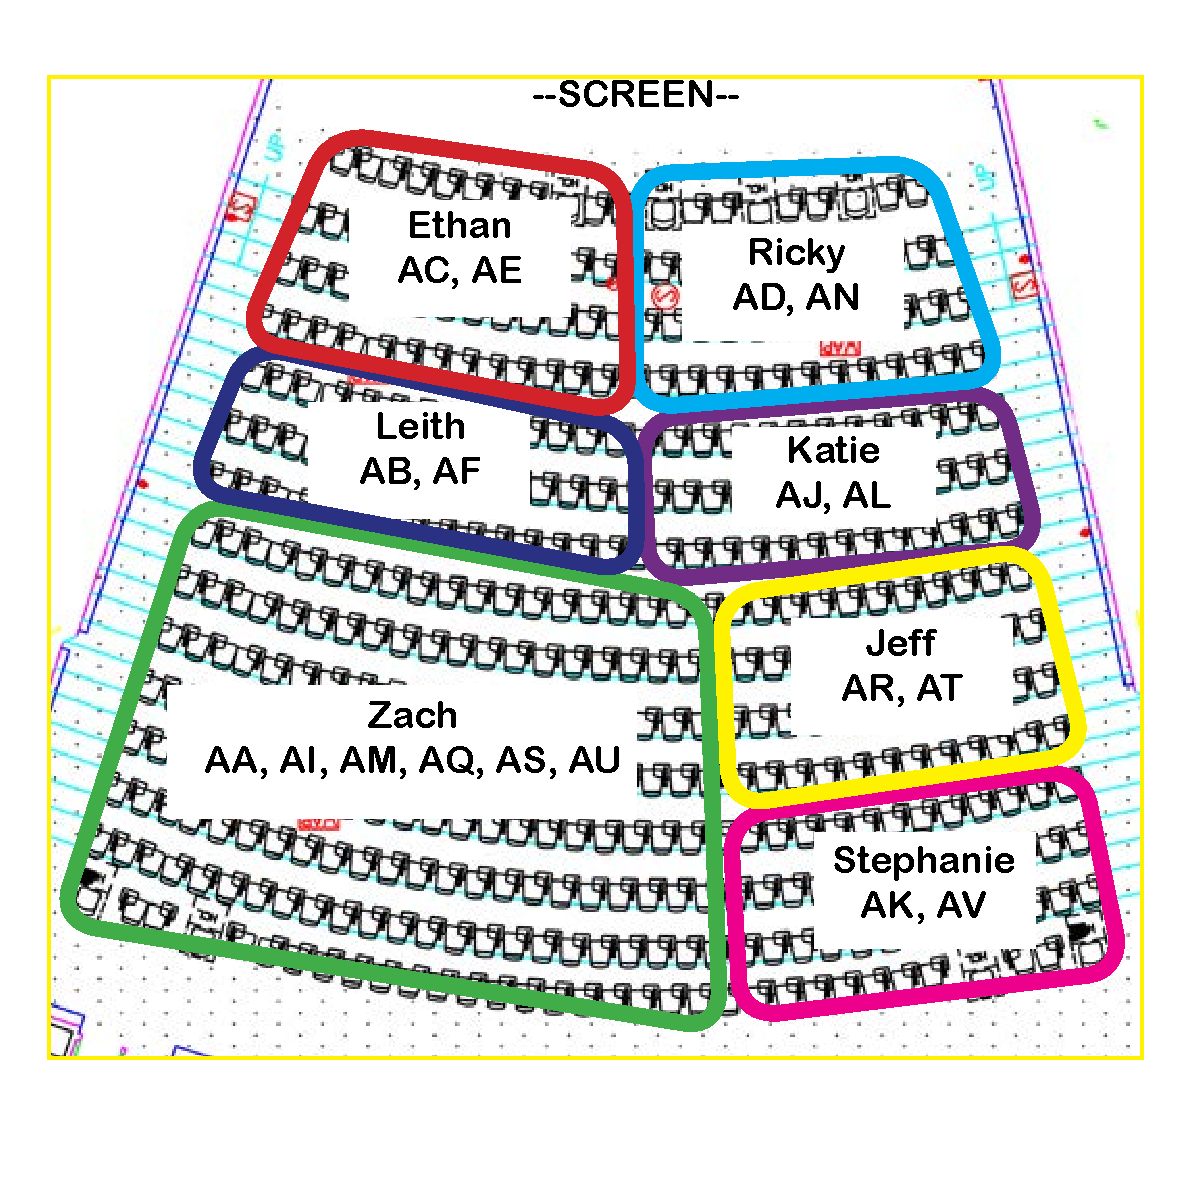
\includegraphics[height=1.2\textheight]{../images/seating-chart.pdf}
    \end{center}
\end{frame}
\end{noheadline}
}

\begin{noheadline}
\begin{frame}
\frametitle{Today's issues:}
\vspace{5mm}
\tableofcontents[subsectionstyle=hide]
\end{frame}
\end{noheadline}

\clickerslide{
\begin{frame}
    \begin{clickerquestion}
        \item In most human populations, average IQ and average height have
            increased significantly over the past 100 years. Which of the
            following is most likely to be correct? 

        \begin{clickeroptions}
            \item The changes in IQ caused the changes in height.
            \item The changes in height caused the changes in IQ. 
            \item \clickeranswer{Both changes were due to gene $\times$
                    environment interactions.}
            \item Both changes were due to changes in allele frequencies.
            \item \clickeranswer{There is not enough information to understand
                    what caused the changes.}
        \end{clickeroptions}
    \end{clickerquestion}
    \nbox{3 and 5 are best, but 4 could also be argued (although the effect
        would be small). The short answer is there's a lot we don't know.}
\end{frame}
}

\section{Constraints on evolution by natural selection}

\begin{noheadline}
\begin{frame}[t]
    \frametitle{Constraints on evolution by natural selection}
    \begin{adjustwidth}{-1.5em}{-1.5em}
        \vspace{-4mm}
        Why doesn't natural selection produce ``perfect'' adaptations?
        
        \begin{uncoverenv}<2->
        \begin{enumerate}
            \item \textbf{Fitness trade-offs}---Why an ``inevitable compromise?''
                
                \begin{uncoverenv}<3->
                \begin{enumerate}
                    \normalsize
                    \item \textbf{Limited resources} \ldots consider:
                        \begin{itemize}
                        \normalsize
                            \item Egg/seed size vs.\ number
                                \nbox{Many small eggs vs.\ few large eggs;
                                    can't have both (many large)!}
                                \vspace{1cm}
                            \item Immune system function vs.\ physical activity
                                \nbox{Energy expended on defense system vs.\
                                    exercise}
                        \end{itemize}
                \end{enumerate}
                \end{uncoverenv}
                \nbox{Inevitable compromise because resources are always
                    limited, and what resources used for one purpose can't be
                    used for another}
        \end{enumerate}
    \end{uncoverenv}
    \end{adjustwidth}
\end{frame}
\end{noheadline}

\clickerslide{
\begin{frame}
    \begin{clickerquestion}
        \item When populations of \textit{D.\ melanogaster} are maintained
            under constant conditions in the lab and selected for shorter or
            longer lifespan, dramatic changes in average lifespan are observed.
            What can you conclude from these experiments? 

        \begin{clickeroptions}
            \item When lifespan changes, average fitness decreases. 
            \item \clickeranswer{Lifespan is a trait with heritable variation.}
            \item Lifespan is driven by gene $\times$ environment interactions.
            \item Lifespan is driven by gene $\times$ gene interactions.
            \item Lifespan is a polygenic trait.
        \end{clickeroptions}
    \end{clickerquestion}

    \nbox{If lifespan can evolve, why wouldn't selection favor longer lifespans
        for all species?}
\end{frame}
}

\begin{noheadline}
\begin{frame}[t]
    \frametitle{Constraints on evolution by natural selection}
    \begin{adjustwidth}{-1.5em}{-1.5em}
        \vspace{-4mm}
        Why doesn't natural selection produce ``perfect'' adaptations?
        
        \begin{enumerate}
            \item \textbf{Fitness trade-offs}---Why an ``inevitable compromise?''
                
                \begin{enumerate}
                    \normalsize
                    \item \textbf{Limited resources} \ldots consider:
                        \begin{itemize}
                        \normalsize
                            \item What is the survival vs.\ reproduction
                                trade-off?
                                \nbox{Continuum of high survival slow
                                    reproduction vs. low survival and rapid
                                    reproduction}
                                \vspace{6mm}
                            \item What type of environment favors long lifespan
                                and slow reproduction?
                                \nbox{Low mortality early in life (high
                                    survivorship) favors living longer and
                                    reproducing over time}
                                \nbox{High mortality (low survivorship)
                                    favors reproducing a lot as quickly as
                                    possible}
                        \end{itemize}
                \end{enumerate}
        \end{enumerate}
    \end{adjustwidth}
\end{frame}
\end{noheadline}

\begin{noheadline}
\begin{frame}[t]
    \frametitle{Constraints on evolution by natural selection}
    \begin{adjustwidth}{-1.5em}{-1.5em}
        \vspace{-4mm}
        Why doesn't natural selection produce ``perfect'' adaptations?
        
        \begin{enumerate}
            \item \textbf{Fitness trade-offs}---Why an ``inevitable compromise?''
                
                \begin{enumerate}
                    \normalsize
                    \addtocounter{enumii}{1}
                    \item \textbf{Physical constraints} \ldots consider:
                        \begin{itemize}
                        \normalsize
                            \item Why can't Boeing make a plane that is fast,
                                maneuverable, fuel efficient, and capable of
                                carrying heavy loads?
                                \nbox{The laws of physics create constraints}
                        \end{itemize}
                \end{enumerate}
        \end{enumerate}
    \end{adjustwidth}
\end{frame}
\end{noheadline}

\begin{noheadline}
\begin{frame}[t]
    \frametitle{Constraints on evolution by natural selection}
    \begin{adjustwidth}{-1.5em}{-1.5em}
        \vspace{-4mm}
        Why doesn't natural selection produce ``perfect'' adaptations?
        
        \begin{enumerate}
            \item \textbf{Fitness trade-offs}---Why an ``inevitable compromise?''
                
                \begin{enumerate}
                    \normalsize
                    \addtocounter{enumii}{2}
                    \item \textbf{Countervailing selection} \ldots consider:
                        \begin{itemize}
                        \normalsize
                            \item Primate brain size
                                \nbox{\small Maternal and fetal mortality creates
                                    selection for smaller brain size}

                                \vspace{4mm}
                            \item Human height
                                \nbox{\small Countervailing selection due to food
                                    (energy) demands, agility, back and neck
                                    problems}
                                % \vspace{2mm}
                            \item Brightly colored feathers in western tanagers
                                \nbox{\small Predation}

                                \vspace{4mm}
                            \item Negative pleiotropy

                                \nbox{\scriptsize Many alleles affect multiple
                                    traits, and thus can be selectively
                                    advantageous for some traits and
                                    deleterious for others}
                        \end{itemize}
                \end{enumerate}
        \end{enumerate}
    \end{adjustwidth}
\end{frame}
\end{noheadline}

\clickerslide{
\begin{frame}
    \begin{clickerquestion}
        \item Big-leaf maples (\textit{Acer macrophyllum}) are very tall and
            have some of the largest leaves found in trees from northern
            latitudes.  Presumably, the large leaf area is advantageous. Why
            aren't the leaves even bigger?

        \begin{clickeroptions}
            \item \clickeranswer{Increased mechanical damage and water loss.}
            \item Photosynthesis wouldn't occur efficiently.
            \item Increased damage from large mammalian herbivores such as deer
                and elk.
            \item Time constraints (not enough time has passed for more
                evolution to occur).
        \end{clickeroptions}
    \end{clickerquestion}
\end{frame}
}

\begin{noheadline}
\begin{frame}[t]
    \frametitle{Constraints on evolution by natural selection}
    \begin{adjustwidth}{-1.5em}{-1.5em}
        \vspace{-4mm}
        Why doesn't natural selection produce ``perfect'' adaptations?
        
        \begin{enumerate}
            \addtocounter{enumi}{1}
            \item \textbf{Historical constraints}
                
                \uncover<2->{
                \begin{enumerate}
                    \normalsize
                    % \addtocounter{enumii}{2}
                    \item \textbf{Selection acts on pre-existing traits} \ldots consider:
                        \begin{itemize}
                        \normalsize
                            \item Cephalopod vs.\ vertebrate eyes

                                \nbox{\scriptsize Both independently evolved
                                    camera-type eye (adjustable lens that
                                    focuses light on retina). We have a blind
                                    spot that certainly has a fitness cost; but
                                    we are constrained by the ancestral
                                    structure of the early vertebrate eye}

                                % \vspace{1.2cm}
                            \item Mammalian middle ear

                                \nbox{\scriptsize Mammals have lost several jaw
                                    bones found in other vertebrates; three of
                                    these were ``re-purposed'' to become the
                                    ossicles of the middle ear}

                                \vspace{5mm}
                            \item Human spine and knees 

                                \nbox{\scriptsize We evolved from a very long
                                    lineage of quadrapeds. Because of this many
                                    of our joints are very poorly ``designed''
                                    for our bipedal posture. E.g., over 93\% of
                                    people suffer from degenerative discs in
                                    their lifetime.}
                        \end{itemize}
                \end{enumerate}
                }
        \end{enumerate}
    \end{adjustwidth}

    \note[item]{Hold index finger up, close left eye, focus right eye on
        location just beyond fingertip \ldots move finger to right \ldots tip
        of index finger vanishes}
\end{frame}
\end{noheadline}

\begin{noheadline}
\begin{frame}[t]
    \frametitle{Constraints on evolution by natural selection}
    \begin{adjustwidth}{-1.5em}{-1.5em}
        \vspace{-4mm}
        Why doesn't natural selection produce ``perfect'' adaptations?
        
        \begin{enumerate}
            \addtocounter{enumi}{1}
            \item \textbf{Historical constraints}
                
                \begin{enumerate}
                    \normalsize
                    % \addtocounter{enumii}{2}
                    \item \textbf{Selection acts on pre-existing traits} \ldots consider:
                        \begin{itemize}
                        \normalsize
                                \vspace{3mm}
                            \item The ``ghost of selection past.'' \\
                            
                                \vspace{3mm}
                                E.g., why do humans love sugar, fat, and
                                    salt so much?

                                \nbox{\small These resources were extremely
                                    rare in the environment until extremely
                                    recently in human evolutionary history. So,
                                    our brain ``rewards us'' for expending
                                    effort to get them and consume as much as
                                    we can. These alleles used to be very
                                    advantageous. Now, they are
                                    deleterious---obesity and type II
                                    diabetes.}

                        \end{itemize}
                \end{enumerate}
        \end{enumerate}
    \end{adjustwidth}

\end{frame}
\end{noheadline}

\section{Common misunderstandings about natural selection}

\begin{noheadline}
\begin{frame}[t]
    \frametitle{Common misconceptions about natural selection}
    \begin{adjustwidth}{-1.5em}{-1.5em}
        \begin{itemize}
            \normalsize
            \item Evolution is progressive---species get larger, more complex,
                and ``better'' over time

                \nbox{Traits (alleles) that increase reproductive success are
                    selected for, whether or not they are ``better'' or more
                    complex.  E.g., evolution of less complexity (e.g., trait
                    loss) is extremely common}

                \vspace{3mm}
            \item The strongest and most socially dominant individuals in a
                population have the highest fitness

                \nbox{\small ``Strong'' and ``socially dominant'' lack meaning for
                    most phenotypes in most environments. Even when they are
                    meaningful, they often don't increase reproductive success
                    (e.g., energy trade-offs, sneaker males)}

                % \vspace{2mm}
            \item Species anticipate changing conditions and adapt to them
                (i.e., evolution is forward looking)

                \nbox{This can't happen---adaptation is always to previous
                    environments (selection in previous generations}
        \end{itemize}
    \end{adjustwidth}
\end{frame}
\end{noheadline}

\begin{noheadline}
\begin{frame}[t]
    \frametitle{Common misconceptions}
    \begin{adjustwidth}{-1.5em}{-1.5em}
        \begin{itemize}
            \normalsize
            \item Evolution is random 

                \nbox{Natural selection is non-random, because individuals with
                    certain alleles (NOT random alleles) produce more offspring
                    than others}

                \vspace{5mm}
            \item Beneficial mutations happen when they are needed (e.g., when
                the environment changes). For example, Ebola virus will undergo
                mutations to make airborne transmission possible.
                
                \nbox{Mutations just happen (they are random). No physical
                    mechanism for them to occur based on need or to be
                    beneficial.}

        \end{itemize}
    \end{adjustwidth}
\end{frame}
\end{noheadline}

\begin{noheadline}
\begin{frame}[t]
    \frametitle{Common misconceptions}
    \begin{adjustwidth}{-1.5em}{-1.5em}
        \begin{itemize}
            \normalsize
            \item Individuals sacrifice themselves for the good of the species

                \nbox{Alleles that cause this behavior would decrease fitness,
                    and would be eliminated by natural selection}

        \end{itemize}
    \end{adjustwidth}
\end{frame}
\end{noheadline}

\clickerslide{
\begin{frame}
    \begin{clickerquestion}
        \item What is wrong with the following statement: ``Species adapt to
            changed environments because they need to in order to persist.''

        \begin{clickeroptions}
            \item It's not about survival. It's about reproduction. 
            \item Species don't adapt---individuals do. 
            \item Frequently, adaptation doesn't occur (species go extinct).
            \item \clickeranswer{There is no need involved---some individuals
                    simply have alleles that give them a reproductive advantage
                    in the current environment.}
        \end{clickeroptions}
    \end{clickerquestion}
\end{frame}
}

\end{document}

\clickerslide{
\begin{frame}
    \begin{clickerquestion}
        \item 
        \begin{clickeroptions}
            \item 
            \item 
            \item 
            \item 
        \end{clickeroptions}
    \end{clickerquestion}
\end{frame}
}
